\documentclass{article}

% ICML 2025 style
\usepackage{icml2025}

% Recommended packages
\usepackage{microtype}
\usepackage{graphicx}
\usepackage{subfigure}
\usepackage{booktabs}
\usepackage{hyperref}
\usepackage{amsmath}
\usepackage{amssymb}

% Attempt to use natbib for \citet support (icml2025 may provide it)
% \usepackage{natbib}

\definecolor{mydarkblue}{rgb}{0,0.08,0.45}
\hypersetup{
    colorlinks=true,
    linkcolor=mydarkblue,
    filecolor=mydarkblue,
    urlcolor=mydarkblue,
    citecolor=mydarkblue,
}

% Use the ICML submission format
\icmltitlerunning{Execution Feedback Dominates Static Analysis for LLM Code Repair}

\begin{document}

\twocolumn[
\icmltitle{Execution Feedback Dominates Static Analysis for LLM Code Repair:\\A Style-Function Dissociation}

\begin{icmlauthorlist}
\icmlauthor{Anonymous}{anon}
\end{icmlauthorlist}

\icmlaffiliation{anon}{Anonymous Institution}

\icmlcorrespondingauthor{Anonymous}{anonymous@institution.edu}

\icmlkeywords{LLM code repair, execution feedback, static analysis, pylint, pass@1, HumanEval, MBPP}

\vskip 0.3in
]

\printAffiliationsAndNotice{}

% Abstract
\begin{abstract}
Iterative code repair---using feedback signals to guide LLM re-generation on failing problems---improves functional correctness, but which feedback signal to use remains an open question. We compare execution test feedback against pylint/mypy static analysis feedback for Llama 3.1 8B Instruct in an iso-compute setting ($B$=1000 output tokens per problem) on HumanEval and MBPP. Execution feedback significantly outperforms pylint/mypy on both benchmarks (McNemar's test: HumanEval $p$=0.0001, MBPP $p$<10$^{-18}$), improving MBPP pass@1 by +40.2pp while pylint/mypy repair actively \emph{reduces} HumanEval pass@1 by $-$4.3pp. The mechanism is a style-function dissociation: pylint flags 100\% of HumanEval failures, but 94.3\% of those flags are Convention-category style rules (missing newlines, missing docstrings) that fire regardless of functional correctness, while functional Error/Warning coverage is only 12.5\%. On complex algorithmic tasks, style-guided rewrites corrupt logical structure; on simpler function-completion tasks (MBPP), they provide marginal benefit. These findings suggest that feedback signal selection for LLM code repair should prioritize functional informativeness over aggregate coverage.
\end{abstract}


% Main sections
\section{Introduction}

When pylint flags 100\% of code failures, you might expect it to guide better repairs. But when 94.3\% of those flags read ``missing newline at end of file'' and ``missing docstring in public module''---universal style complaints that fire on virtually every snippet of LLM-generated code regardless of whether the code is correct---the model receiving this feedback is being told to fix formatting on code that fails for logical reasons. The result, as we show empirically, is not neutral: on HumanEval's algorithmic problems, pylint-guided repair actively \emph{decreases} pass@1 by 4.3 percentage points, producing a model that performs worse after repair than before.

This counterintuitive finding motivates our study. Iterative code repair---generating code, receiving feedback on failures, and re-generating to fix them---has emerged as a practical approach to improving LLM code quality at inference time \cite{Chen2023Teaching, Shinn2023Reflexion, Arimbur2026HowMany}. The key question for practitioners is which feedback signal to use: execution test results (run the code, observe failures), static analysis (run pylint/mypy, observe warnings), or constrained decoding (prevent certain errors at generation time). Each approach has been studied in isolation, but no prior work provides a compute-controlled, head-to-head comparison of execution vs.\ pylint/mypy feedback on functional correctness benchmarks with mechanistic analysis of \emph{why} one signal outperforms the other.

The surface problem is straightforward: LLMs generate incorrect code (39\% failure rate on HumanEval, 67\% on MBPP for a competitive 7B model), and feedback-based repair can help. The deeper problem is that feedback signals differ in \emph{informativeness}---how well they diagnose the specific errors present in a failure. Static analysis tools like pylint were designed to enforce code style conventions and detect syntactically suspicious patterns; they were not designed to detect the logical and runtime errors that dominate HumanEval and MBPP failures. The critical gap is that no study has measured this informativeness difference empirically under compute-controlled conditions, nor decomposed \emph{which} pylint signals are informative vs.\ noise for functional correctness repair.

Our key insight is that pylint and mypy achieve high \emph{coverage} of LLM code failures---flagging every failing program---but the dominant signals are Convention-category style rules (C0304: missing newline, C0114: missing docstring) that fire universally on LLM output regardless of correctness. Only 12.5\% of failures receive a functional Error or Warning flag. This style-function dissociation explains both why pylint feedback fails to match execution feedback overall and why it actively harms performance on complex algorithmic tasks: the LLM, following style guidance, may restructure solutions while introducing new logical errors.

Building on this insight, we make the following contributions:

\textbf{C1: First iso-compute comparison of execution vs.\ pylint/mypy feedback.} We compare execution test feedback against pylint/mypy static analysis feedback at a fixed token budget of $B$=1000 output tokens per problem on HumanEval (164 problems) and MBPP (378 problems) using Llama 3.1 8B Instruct. Our paired McNemar test confirms execution feedback is significantly superior on both benchmarks (HumanEval: $p$=0.0001, MBPP: $p$<10$^{-18}$), with 15 problems uniquely repaired by execution vs.\ zero by pylint on HumanEval, and 85 vs.\ 2 on MBPP.

\textbf{C2: Novel style-function dissociation measurement.} We decompose pylint flags by category (E/W/C/R/I) across 64 HumanEval baseline failures and show that 94.3\% are Convention-category style flags (C0304, C0114) that fire regardless of functional correctness, while only 12.5\% are functional Error or Warning flags. Mypy coverage is 0\%, confirming that type errors are not the dominant failure mode. This decomposition reveals that coverage without category analysis systematically overstates feedback informativeness.

\textbf{C3: Benchmark asymmetry and task-complexity moderation.} Pylint/mypy repair harms HumanEval ($\Delta$=$-$4.3pp) but benefits MBPP ($\Delta$=+18.3pp), while execution feedback improves both. We interpret this asymmetry as task-complexity moderation: MBPP's simpler function-completion tasks tolerate style-guided rewrites without losing logical structure, whereas HumanEval's algorithmic problems are sensitive to rewriting triggered by style feedback.

We organize the paper as follows. Section~\ref{sec:related} reviews related work on feedback-driven code repair and positions our contribution. Section~\ref{sec:methodology} describes our iso-compute experimental methodology. Section~\ref{sec:setup} presents our experimental setup. Section~\ref{sec:results} reports results. Section~\ref{sec:discussion} discusses implications, limitations, and future work. Section~\ref{sec:conclusion} concludes.

\section{Related Work}
\label{sec:related}

\subsection{Execution Feedback for Iterative Code Repair}

Iterative self-repair using execution feedback---generate code, execute it, use error output as context, re-generate---is a well-established approach. \citet{Chen2023Teaching} showed that execution trace feedback enables LLMs to self-debug, improving MBPP by 12\% and achieving 10$\times$ sample efficiency compared to best-of-N sampling. \citet{Shinn2023Reflexion} demonstrated that verbal reinforcement via execution results reaches 91\% HumanEval pass@1 in Reflexion. \citet{Gehring2024RLEF} showed that RL-grounded execution feedback (RLEF) further improves over prompting-only repair, reducing required samples by 10$\times$. Most recently, \citet{Arimbur2026HowMany} showed that modern 8B instruction-tuned models---including Llama 3.1 8B---achieve meaningful self-repair (+4.9 to +17.1pp HumanEval) with execution feedback alone, without fine-tuning, and that most gains occur in repair rounds 1--2.

These works collectively establish that execution feedback \emph{works}. However, none compare execution feedback against pylint/mypy static analysis on the same benchmarks under compute-controlled conditions. Our work fills this gap.

\subsection{Static Analysis Feedback for LLM Code Quality}

Pylint, mypy, and related static analysis tools have been integrated into LLM code generation pipelines primarily for quality metrics beyond functional correctness. \citet{Blyth2025Static} demonstrated that iterative pylint/bandit feedback reduces security issues in LLM-generated code from 40\% to 13\% over 10 iterations on PythonSecurityEval. This result establishes that pylint \emph{can} provide useful feedback---but on a benchmark where pylint's Error and Warning categories (security violations) are the dominant failure mode. HumanEval and MBPP failures are dominated by logic and runtime errors, not security issues, making this result difficult to generalize.

FeedbackEval \cite{Dai2025FeedbackEval} provides the most systematic comparison of feedback types, covering compiler feedback, test feedback, minimal feedback, and LLM-expert feedback across HumanEval, CoderEval, and SWE-bench. However, FeedbackEval excludes semantic static analysis (pylint/mypy)---it uses compiler output (syntax errors) rather than pylint-style warnings---and does not compare against execution test feedback with compute normalization. Our study directly addresses this gap: we add pylint/mypy as a treatment condition and hold token budget constant across all conditions.

\subsection{Type-Constrained Decoding}

\citet{Mundler2025Type} showed that type-constrained decoding---enforcing type correctness via vocabulary-filtered generation---reduces compilation errors by over 50\% on HumanEval and MBPP. This approach is fundamentally different from repair-mode feedback: it prevents certain errors at generation time rather than correcting them after. As a \emph{prevention} strategy, it is not directly comparable to iterative repair.

\subsection{Positioning Our Work}

Our study differs from prior work in three ways: (1) head-to-head pylint/mypy vs.\ execution comparison on the same benchmarks; (2) iso-compute control ($B$=1000 output tokens per problem across all conditions); (3) mechanism analysis decomposing pylint coverage by flag category.

\section{Methodology}
\label{sec:methodology}

\subsection{Overview}

Our study addresses a fundamental question in LLM code repair: which feedback signal---execution test results or pylint/mypy static analysis warnings---produces larger pass@1 improvement when both are given the same inference compute budget? The iso-compute constraint is the methodological core: without it, apparent feedback quality differences may simply reflect differences in the number of tokens spent on repair.

\subsection{Experimental Conditions}

We compare three conditions on HumanEval (164 problems) and MBPP (378 problems):

\textbf{Condition A: No-feedback baseline.} Single-pass greedy decoding. No repair. All token budget $B$ spent on initial generation.

\textbf{Condition B: Pylint/mypy iterative repair.} After initial generation, failing solutions receive pylint and mypy output formatted as structured feedback. The LLM re-generates given the original problem + failed solution + feedback. Repair continues until the token budget is exhausted.

\textbf{Condition C: Execution test feedback iterative repair.} After initial generation, failing solutions are executed against the benchmark test suite. The error output (exception type, traceback, expected vs.\ actual values) is formatted as structured feedback. The LLM re-generates given the original problem + failed solution + execution feedback.

\textbf{Key invariant:} All conditions use Llama 3.1 8B Instruct, greedy decoding (temperature=0, seed=42), and token budget $B$=1000 output tokens per problem.

\subsection{Iso-Compute Token Budget}

The token budget $B$=1000 output tokens per problem is the experimental unit of compute. Repair stops when the remaining budget falls below 50 tokens or when the problem passes. At $B$=1000, with \texttt{max\_tokens}=512 per round and initial generation consuming approximately 400--512 tokens, most problems complete one repair round before budget exhaustion. Per-round trajectory data confirms that rounds 2--3 contribute near-zero incremental improvement.

\subsection{Feedback Signal Design}

\textbf{Pylint/mypy feedback format.} We run \texttt{pylint --output-format=text} (default configuration, all categories) and \texttt{mypy} on each failing solution. Output is parsed and formatted as structured prompt context.

\textbf{Execution feedback format.} We execute the failing solution in a sandboxed subprocess (15-second timeout) against the benchmark's test assertions. The exception type, traceback ($\leq$512 chars), and first failing assertion are formatted as structured feedback.

\subsection{Statistical Analysis}

\textbf{Primary test: McNemar's test} on the paired 2$\times$2 contingency table (condition-passes $\times$ condition-fails), $\alpha$=0.05.

\textbf{Effect size: $\Delta_{\text{pass@1}}$} = pass@1(condition) $-$ pass@1(no-feedback baseline).

\textbf{Bootstrap CIs:} 95\% confidence intervals, 10,000 samples, seed=42.

\subsection{Mechanism Study: Pylint Coverage Analysis}

For the 64 HumanEval baseline failures, we run pylint and mypy and record all flags by category (E: Error, W: Warning, C: Convention, R: Refactor, I: Information). We compute total coverage, functional coverage (E+W), and the category distribution of all flags.

\subsection{Model and Infrastructure}

\begin{table}[h]
\centering
\caption{Model and infrastructure parameters.}
\label{tab:infra}
\begin{tabular}{ll}
\toprule
\textbf{Parameter} & \textbf{Value} \\
\midrule
Model & Llama 3.1 8B Instruct \\
Backend & vLLM v0.10.1.1 (bfloat16) \\
Hardware & 5$\times$ H100 NVL \\
Token budget $B$ & 1000 output tokens per problem \\
Max repair rounds & 3 (effectively 1 at $B$=1000) \\
Execution timeout & 15 seconds \\
\bottomrule
\end{tabular}
\end{table}

\section{Experimental Setup}
\label{sec:setup}

\subsection{Research Questions}

\textbf{RQ1:} Does execution test feedback achieve significantly larger pass@1 improvement than pylint/mypy at fixed $B$=1000?

\textbf{RQ2:} What fraction of HumanEval failures does pylint/mypy detect, and which flag categories dominate?

\textbf{RQ3:} Does the execution advantage vary by benchmark complexity?

\subsection{Datasets}

\textbf{HumanEval} \cite{Chen2021Evaluating}: 164 algorithmic programming problems. Baseline pass@1: 61.0\% (64/164 failures).

\textbf{MBPP} \cite{Austin2021Program}: 378 function-completion problems (EvalPlus format). Baseline pass@1: 33.1\% (253/378 failures).

\begin{table}[h]
\centering
\caption{Dataset statistics.}
\label{tab:datasets}
\begin{tabular}{llll}
\toprule
\textbf{Dataset} & \textbf{\# Problems} & \textbf{Failure Rate} & \textbf{Problem Type} \\
\midrule
HumanEval & 164 & 39\% (64/164) & Algorithmic reasoning \\
MBPP & 378 & 67\% (253/378) & Function completion \\
\bottomrule
\end{tabular}
\end{table}

\subsection{Evaluation Metrics}

\textbf{Primary:} $\Delta_{\text{pass@1}}$ per condition; McNemar's test ($\alpha$=0.05).

\textbf{Mechanism:} Pylint total and functional (E+W) coverage fraction over HumanEval failures. Bootstrap 95\% CI.

\textbf{Secondary:} Per-round pass@1 trajectory (rounds 0--3).

\section{Results}
\label{sec:results}

\subsection{Main Comparison: Execution vs.\ Pylint/Mypy (RQ1)}

Execution feedback significantly outperforms pylint/mypy feedback on both benchmarks. Figure~\ref{fig:delta} shows the pass@1 improvement delta with 95\% bootstrap confidence intervals.

\begin{table}[h]
\centering
\caption{Main results: pass@1 and improvement delta ($\Delta$) per condition.}
\label{tab:main}
\begin{tabular}{lllll}
\toprule
\textbf{Condition} & \textbf{HE pass@1} & \textbf{$\Delta_{\text{HE}}$} & \textbf{MBPP pass@1} & \textbf{$\Delta_{\text{MBPP}}$} \\
\midrule
No-feedback (baseline) & 61.0\% & --- & 33.1\% & --- \\
Pylint/mypy repair & 56.7\% & $-$4.3pp & 51.4\% & +18.3pp \\
Execution feedback & 65.9\% & \textbf{+4.9pp} & 73.3\% & \textbf{+40.2pp} \\
\bottomrule
\end{tabular}
\end{table}

The most striking result is on MBPP: a single round of execution feedback repair improves pass@1 from 33.1\% to 73.3\%---a +40.2pp absolute improvement, more than doubling the baseline success rate.

\begin{table}[h]
\centering
\caption{McNemar test results: problems exclusively repaired by each condition.}
\label{tab:mcnemar}
\begin{tabular}{llll}
\toprule
\textbf{Benchmark} & \textbf{Exec-only} & \textbf{Pylint-only} & \textbf{McNemar $p$-value} \\
\midrule
HumanEval & 15 & 0 & $p$ = 0.0001 \\
MBPP & 85 & 2 & $p$ < 10$^{-18}$ \\
\bottomrule
\end{tabular}
\end{table}

On HumanEval, 15 problems are exclusively repaired by execution feedback---zero are exclusively repaired by pylint. On MBPP, 85 problems are exclusively repaired by execution vs.\ 2 by pylint.

\begin{figure}[h]
\centering
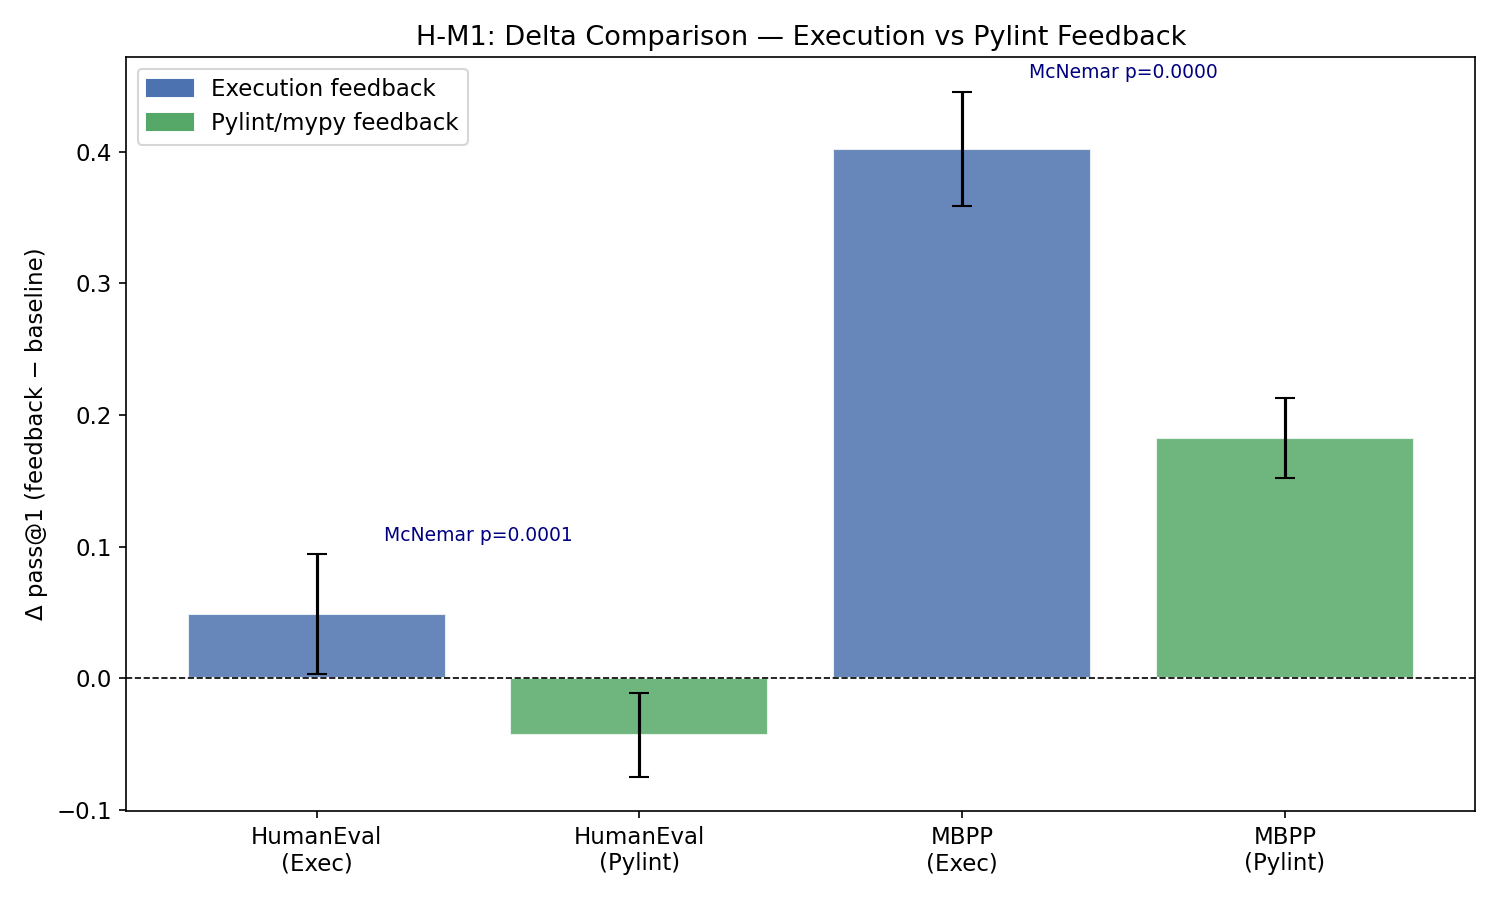
\includegraphics[width=0.85\columnwidth]{figures/figure1_delta_comparison.png}
\caption{Pass@1 improvement delta ($\Delta$) with 95\% bootstrap CIs and McNemar $p$-values for both benchmarks. Execution feedback (blue) significantly outperforms pylint/mypy (orange) on both HumanEval and MBPP.}
\label{fig:delta}
\end{figure}

\begin{figure}[h]
\centering
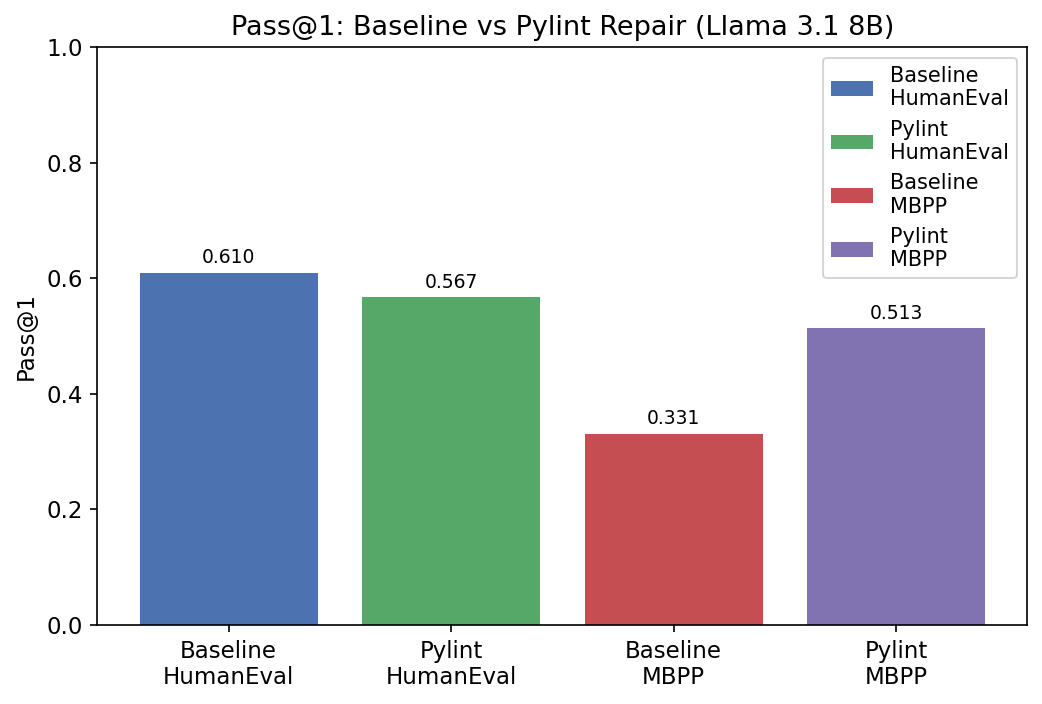
\includegraphics[width=0.85\columnwidth]{figures/figure1_pass_at_1_comparison.png}
\caption{Absolute pass@1 values for all three conditions on both benchmarks.}
\label{fig:absolute}
\end{figure}

\subsection{Pylint/Mypy Coverage Analysis---The Mechanism (RQ2)}

\textbf{Coverage result:} Pylint/mypy flags 100\% of the 64 HumanEval baseline failures (bootstrap CI: [100\%, 100\%]).

\begin{table}[h]
\centering
\caption{Pylint flag category distribution across 64 HumanEval failures (300 total flags).}
\label{tab:pylint}
\begin{tabular}{lllll}
\toprule
\textbf{Category} & \textbf{Flags} & \textbf{Fraction} & \textbf{Type} \\
\midrule
C (Convention) & 283 & 94.3\% & Style (C0304, C0114) \\
R (Refactor) & 8 & 2.7\% & Style/structure \\
W (Warning) & 7 & 2.3\% & Functional \\
E (Error) & 1 & 0.3\% & Functional \\
I (Information) & 1 & 0.3\% & Informational \\
\bottomrule
\end{tabular}
\end{table}

\textbf{Functional coverage (E+W):} 8/64 failures = 12.5\% (8 distinct failures receiving at least one Error or Warning flag; the single I-category flag is informational, not functional). Mypy coverage: 0/64 = 0\%.

The 100\% total coverage is driven by C0304 (``missing newline at end of file'') and C0114 (``missing docstring in public module'')---properties of LLM code generation context, not indicators of logical errors.

\begin{figure}[h]
\centering
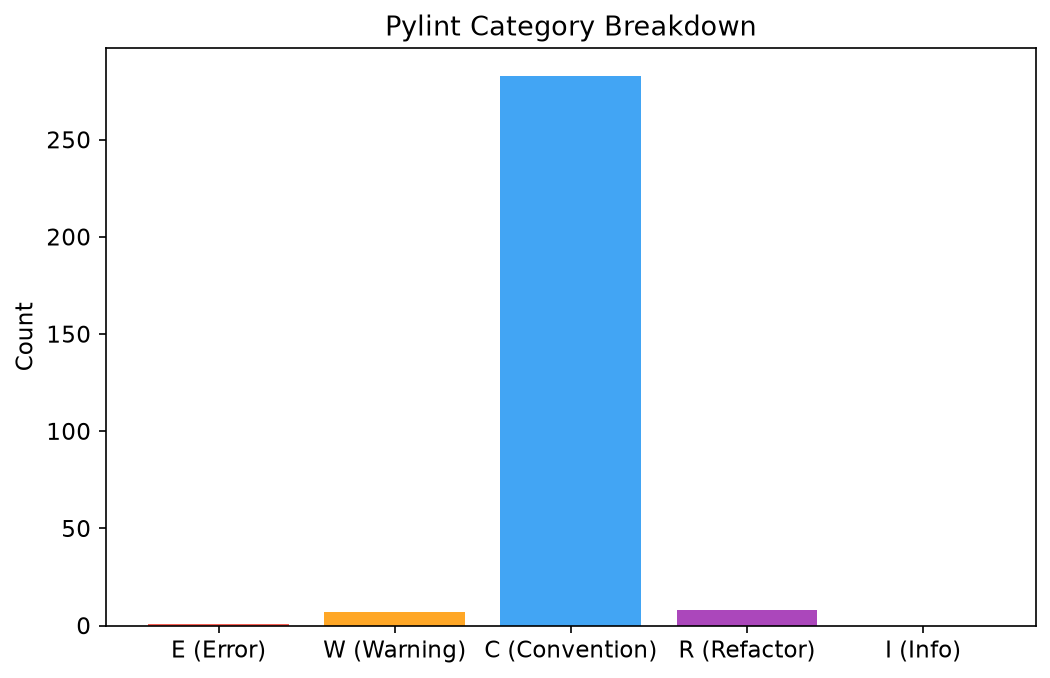
\includegraphics[width=0.85\columnwidth]{figures/fig2_pylint_categories.png}
\caption{Pylint flag category distribution across 64 HumanEval failures. The 94.3\% Convention-category dominance (C0304, C0114) reveals the style-function dissociation: pylint's high coverage is driven by style rules orthogonal to functional correctness.}
\label{fig:categories}
\end{figure}

\begin{figure}[h]
\centering
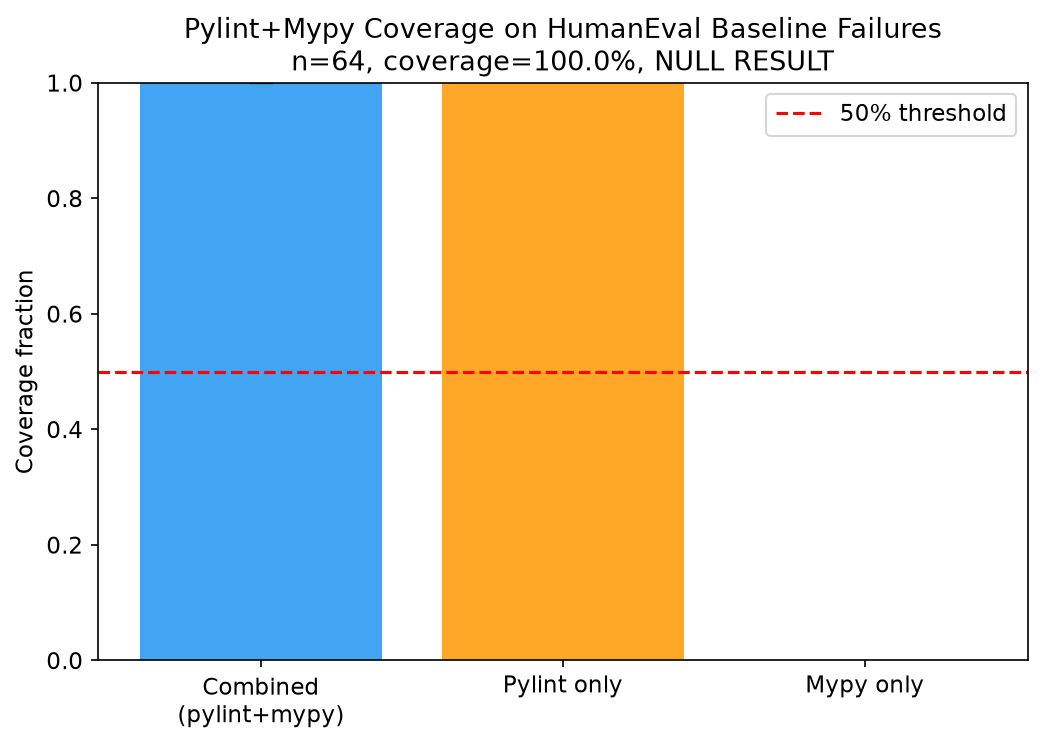
\includegraphics[width=0.85\columnwidth]{figures/fig1_coverage_bar.png}
\caption{Total pylint/mypy coverage (100\%) vs.\ functional coverage (E+W only, 12.5\%) with 95\% bootstrap confidence intervals across HumanEval baseline failures.}
\label{fig:coverage}
\end{figure}

\subsection{Benchmark Asymmetry and Task-Complexity Moderation (RQ3)}

Pylint repair hurts HumanEval ($-$4.3pp) but helps MBPP (+18.3pp). We interpret this as task-complexity moderation: MBPP's simpler function-completion tasks tolerate style-guided rewrites without losing logical structure; HumanEval's algorithmic problems are sensitive to rewriting triggered by style feedback.

\begin{figure}[h]
\centering
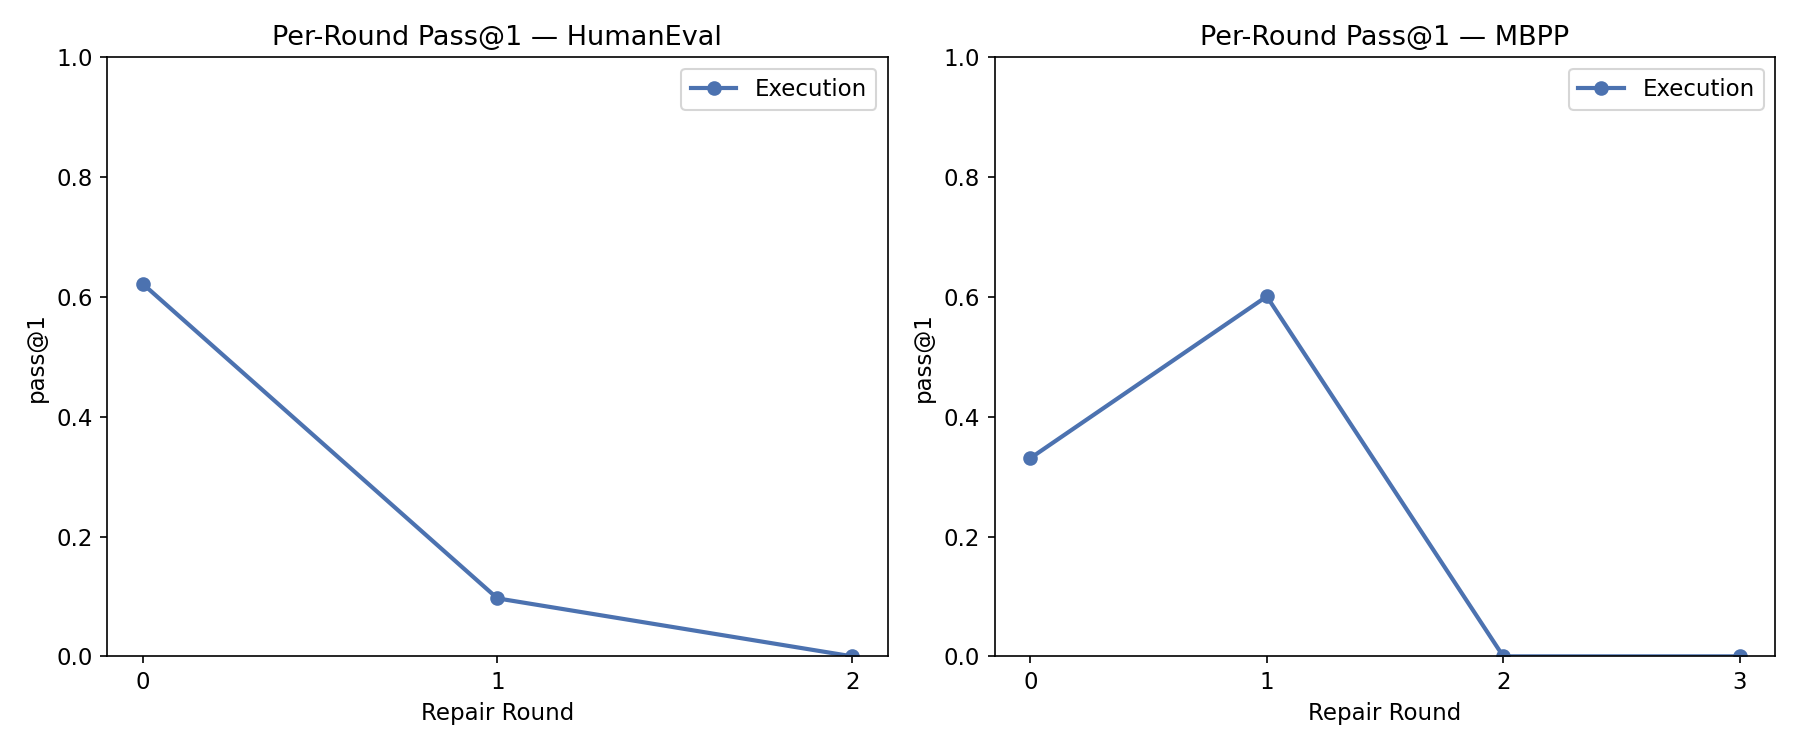
\includegraphics[width=0.85\columnwidth]{figures/figure2_per_round_trajectory.png}
\caption{Per-round pass@1 trajectory (rounds 0--3) for execution feedback condition, confirming round-1 dominance at $B$=1000.}
\label{fig:trajectory}
\end{figure}

\subsection{Budget Saturation}

At $B$=1000, the token budget is effectively exhausted after round 1 for most problems. Figure~\ref{fig:trajectory} confirms that rounds 2--3 contribute near-zero incremental improvement. Results characterize \textbf{single-round repair at $B$=1000}. Note: Round 0 in Figure~\ref{fig:trajectory} represents the initial generation pass@1 within the execution feedback condition's experimental run and may differ slightly from the no-feedback baseline (61.0\%) due to prompt-context differences; the no-feedback baseline is a separate single-pass condition without any repair loop instrumentation.

\section{Discussion}
\label{sec:discussion}

\subsection{Key Findings}

\textbf{Finding 1: Style-function dissociation as the primary mechanism.} Coverage without category analysis is misleading: pylint's 100\% total coverage of HumanEval failures overstates its diagnostic value. The 94.3\% C-category dominance means the LLM receives ``fix your formatting'' as its primary repair guidance on algorithmic failures. On complex tasks, this style-triggered rewriting corrupts logical structure, explaining the HumanEval regression. Future work reporting pylint coverage of LLM failures should decompose by flag category.

\textbf{Finding 2: Execution feedback is practically effective at fixed compute.} The +40.2pp MBPP improvement from a single round at $B$=1000 is substantively large---more than doubling baseline performance on a standard benchmark at minimal inference cost. The +4.9pp HumanEval improvement is smaller but robust. Execution feedback is a reliable choice for single-round repair across benchmark types.

\textbf{Finding 3: Task complexity moderates static analysis feedback utility.} Even low-information-content feedback (94.3\% style flags) helps on MBPP's simple tasks (+18.3pp). Style-guided rewrites preserve logical structure in short functions; they disrupt it in complex algorithms. The appropriate feedback signal may depend on the complexity profile of target tasks.

\subsection{Limitations}

\textbf{L1: Single model.} Results are based on Llama 3.1 8B Instruct only. Qwen2.5-Coder-7B replication was planned but not executed (resource constraints). Claims are scoped to Llama 3.1 8B.

\textbf{L2: Single repair round.} At $B$=1000, most problems complete one repair round. Results characterize single-round repair, not multi-round iterative improvement. Per-round data confirms this captures the primary effect.

\textbf{L3: P2 prediction refuted (informative null).} We predicted pylint coverage $<$50\%; actual coverage was 100\%. This null result on the primary metric is reported transparently. The functional coverage result (12.5\% E+W) is arguably more informative than the original prediction.

\textbf{L4: No per-problem qualitative analysis.} The ``style-guided corruption'' mechanism is inferred from aggregate results, not confirmed by per-problem solution comparison.

\subsection{Broader Impact}

This work contributes to responsible deployment of LLM-based code generation tools. Production systems using static analysis as repair feedback should be evaluated on functional correctness, not just coverage. The style-function dissociation may be invisible in aggregate quality metrics but visible in pass@k evaluations. No significant negative societal impacts are identified from this benchmarking study.

\section{Conclusion}
\label{sec:conclusion}

We began by observing a coverage paradox: pylint flags 100\% of HumanEval baseline failures, yet pylint-guided repair \emph{reduces} HumanEval pass@1 by 4.3 percentage points. Our study shows that this paradox resolves cleanly once coverage is decomposed by flag category. The 100\% coverage is a mirage---it is driven by Convention-category style rules (C0304: missing newline, C0114: missing docstring) that fire universally on LLM-generated code regardless of functional correctness. Only 12.5\% of HumanEval failures receive a functional (Error or Warning category) flag; mypy coverage is 0\%. When the LLM receives ``fix your formatting'' as its primary repair guidance on a failed algorithmic solution, it may restructure code while addressing style---and on complex HumanEval problems, this rewriting introduces new logical errors.

Our main contributions are: (1) first iso-compute comparison confirming execution feedback significantly dominates pylint/mypy on HumanEval and MBPP (McNemar $p$=0.0001 and $p$<10$^{-18}$); (2) style-function dissociation measurement (94.3\% C-category, 12.5\% E+W functional coverage); (3) benchmark asymmetry finding revealing task-complexity moderation of static analysis feedback utility.

\textbf{Future directions.} Qwen2.5-Coder-7B replication; per-problem solution analysis for regression cases; W+E-only pylint filtering (removing C-category noise); larger budget comparison ($B$=2000+) for multi-round characterization; extension to code-specialized models and non-Python benchmarks.

For LLM code repair, the question is not whether a tool detects errors---it is whether it detects the \emph{right} errors. Pylint detects formatting; execution detects failure. At $B$=1000 on functional correctness benchmarks, the difference is +40.2pp on MBPP.


% References
\bibliography{references}
\bibliographystyle{icml2025}

\end{document}
